% !TEX encoding = UTF-8 Unicode
% !TEX program = xelatex

\documentclass[
    11pt, % Set the default font size, options include: 8pt, 9pt, 10pt, 11pt, 12pt, 14pt, 17pt, 20pt
    aspectratio=169, % Set the aspect ratio to a 16:9 ratio which matches the aspect ratio of 1080p and 4K screens and projectors
]{beamer}
\usepackage[american, russian]{babel}
\usepackage{fontspec}
\setmainfont{Arial}
\setsansfont{Calibri}
\def\contentsname{Оглавление}%


% This template is inspired by the VT Presentation Template, as well as the THU Beamer Theme. Many thanks!

\graphicspath{{images/}{./}} % Specifies where to look for included images (trailing slash required)
\usepackage{booktabs} % Allows the use of \toprule, \midrule and \bottomrule for better rules in tables
%\usepackage{calligra} % Font for wordart
% \usepackage{appendixnumberbeamer} % If you want a separate slide counter for your appendix
\usepackage{fnpct} % Eliminate the unwanted space before the footnote mark
\usepackage{listings} % For code display
\usepackage{physics}

%---------------------------------------------------------
%	FOOTNOTES & CITATIONS BASIC SETUP
%---------------------------------------------------------
% Check FOOTNOTES & CITATIONS ADVANCED SETUP for solutions for intra- and inter-frame citations
% The workarounds in ADVANCED SETUP require the style to be "numeric"
% If you're good without ADVANCED SETUP, comment out the ADVANCED SETUP section, and pick whatever style you like
% \usepackage[style=authoryear, backend=bibtex]{biblatex}
\usepackage[style=numeric, sorting=none, backend=biber]{biblatex}
\addbibresource{bib.bib}
\setbeamerfont{footnote}{size=\tiny}
% The lines below set the citation style to "number, title, year". The ADVANCED SETUP will overwrite this style
\usepackage{xpatch}
\xapptobibmacro{cite}{\setunit{\nametitledelim} \printfield{title} \setunit{\nametitledelim} \printfield{year}}

%---------------------------------------------------------
%	FOOTNOTES & CITATIONS ADVANCED SETUP
%---------------------------------------------------------
% Manage faulty intra- and inter-frame footnotes and citations. References:
%     https://tex.stackexchange.com/a/520777
%     https://topanswers.xyz/tex?q=453

% You might want to use \firstcite and \secondcite instead of \footnote in your document
% Mark the first citation with \firstcite and the rest with \secondcite

% \renewcommand{\thefootnote}{\arabic{footnote}} % Switch to footnote with numbers
% \renewcommand{\thefootnote}{\alph{footnote}} % Switch to footnote with letters

\DeclareCiteCommand{\firstcite}
{\usebibmacro{prenote}}
{%
    \footnotemark[\thefield{labelnumber}]% mark corresponding to the number entry
    \footnotetext[\thefield{labelnumber}]{% footnote text corresponding to the number entry
        \printnames{labelname}% name
        \setunit{\printdelim{nametitledelim}}% separator
        % \setunit{\addperiod\space}% another way to add separator
        \printfield[citetitle]{labeltitle}% title
        \setunit{\printdelim{nametitledelim}}% separator
        \printfield{year}% year
        \newunit{\adddot}% ending dot
    }%
}
{\multicitedelim}
{\usebibmacro{postnote}}

\DeclareCiteCommand{\secondcite}
{\usebibmacro{prenote}}
{%
    \footnotemark[\thefield{labelnumber}]% mark corresponding to the number entry
}
{\multicitedelim}
{\usebibmacro{postnote}}

%---------------------------------------------------------
%	SELECT THEME & COLORS
%---------------------------------------------------------
\usetheme{Madrid} % You can use other themes too, but this changes many things. I've found Madrid to be the best for this color scheme

% fg = foreground color
% bg = background color

% Many colors are linked to multiple attributes, change with caution!
\definecolor{smuBlue}{RGB}{0,86,145}
%\definecolor{smuGold}{RGB}{138, 112, 76}
\definecolor{scisGold}{RGB}{255, 140, 0}

\setbeamercolor*{structure}{bg=smuBlue, fg=smuBlue}
% Title block and bottom right box color
\setbeamercolor*{palette primary}{use=structure, fg=white,bg=smuBlue} % Bottom left box and bar between title & top bubbles
\setbeamercolor*{palette secondary}{use=structure, fg=smuBlue, bg=white}
% Probably not used
\setbeamercolor*{palette tertiary}{use=structure, fg=white, bg=smuBlue} 

% Title of each slide
\setbeamercolor{frametitle}{bg=smuBlue, fg=white}
\setbeamercolor*{titlelike}{parent=palette primary}

%%% Headline and Central Footer %%%
% You can change the theme back and forth for each frame
% Theme I - white head, white foot
    % \setbeamercolor{section in head/foot}{fg=scisGold, bg=white}
    % \setbeamercolor{headline}{fg=scisGold, bg=white}
% Theme II - gold head, gold foot (as shown in the title frame)
    \setbeamercolor{section in head/foot}{fg=black, bg=scisGold}
    \setbeamercolor{headline}{fg=white, bg=scisGold}
% Theme III - white head, gold foot (as shown in the rest of the frames)
    % \setbeamercolor{section in head/foot}{fg=scisGold, bg=white}
    % \setbeamercolor{title in head/foot}{fg=white, bg=scisGold}
    % \setbeamercolor{headline}{fg=scisGold, bg=white}

%%% Specific Colors %%%
\setbeamercolor{item projected}{bg=scisGold}
\setbeamertemplate{enumerate items}{bg=scisGold}

\setbeamercolor{itemize item}{fg=scisGold}
\setbeamercolor{itemize subitem}{fg=scisGold}

\setbeamercolor{button}{bg=scisGold}

%%% Edits ONLY the TOC slide %%%
\setbeamercolor{section in toc}{fg=black}
\setbeamercolor{subsection in toc}{fg=black}

%%% Block Colors %%%
% Standard block
    \setbeamercolor{block title}{bg=scisGold, fg=white}
    \setbeamercolor{block body}{bg=scisGold!20}
% Alerted block
    \setbeamercolor{block title alerted}{bg=orange, fg=white}
    \setbeamercolor{block body alerted}{bg=orange!10}
% Example block
    \setbeamercolor{block title example}{bg=smuBlue, fg=white}
    \setbeamercolor{block body example}{bg=smuBlue!10}

%---------------------------------------------------------
%	SELECT THE FONT THEME & FONTS
%---------------------------------------------------------
\usefonttheme{default} % Typeset using the default sans serif font
%\usepackage{palatino} % Use the Palatino font for serif text
%\usepackage[default]{opensans} % Use the Open Sans font for sans serif text
\useinnertheme{circles}

%---------------------------------------------------------
%	SELECT THE OUTER THEME
%---------------------------------------------------------
% Outer themes change the overall layout of slides, such as header and footer lines, sidebars and slide titles. Uncomment each theme in turns to see what changes it makes to your presentation.

%\useoutertheme{default}
\useoutertheme{miniframes}
%\usepackage{ulem}
%\useoutertheme{infolines}
 %\useoutertheme{smoothbars}
 %\useoutertheme{sidebar}
 %\useoutertheme{split}
 %\useoutertheme{shadow}
 %\useoutertheme{tree}
 %\useoutertheme{smoothtree}

%---------------------------------------------------------
%	PRESENTATION INFORMATION
%---------------------------------------------------------
\title[Дуальная магнитооптическая структура]{Дуальная магнитооптическая структура\\ для лёгких и тяжёлых частиц}
% Click the middle footer can switch between the first and last numbered frame
%\subtitle{XHU}
\author[Колокольчиков C., Сеничев Ю., Аксентьев А., Мельников А.]{Колокольчиков С.Д.\textsuperscript{1}*, Сеничев Ю.В.\textsuperscript{1}, Аксентьев А.E.\textsuperscript{1,2}, Мельников А.А.\textsuperscript{1,3}}

\institute[]{
\textsuperscript{1}Институт Ядерных Исследований РАН, Москва, Россия\\
\textsuperscript{2}Национальный исследовательский ядерный университет МИФИ, Москва, Россия\\
\textsuperscript{3}Институт теоретической физики им. Л.Д. Ландау, Черноголовка, Россия
 \\ \smallskip *sergey.bell13@gmail.com}
\date[28 января 2025]
% \date[\today]

% School logo
% You can enable and disable logo display for each frame
\logo{
\includegraphics[width=1cm]{logo.eps}}

%---------------------------------------------------------
%	CODE DISPLAY
%---------------------------------------------------------
\lstset{
    basicstyle=\ttfamily\small,
    keywordstyle=\bfseries\color{blue},
    emphstyle=\ttfamily\color{red},   
    stringstyle=\color{green},
    numbers=left,
    numberstyle=\small\color{gray},
    rulesepcolor=\color{red!20!green!20!blue!20},
    frame=shadowbox,
    xleftmargin=1cm,
    xrightmargin=1cm,
}

%---------------------------------------------------------
%	EXTRA SETTINGS
%---------------------------------------------------------

% Clear warnings related to \translate
%     https://github.com/josephwright/beamer/issues/449
\pdfstringdefDisableCommands{
    \def\translate#1{#1}
}

% Adjust header height
\setbeamertemplate{headline}{
    \nointerlineskip
    \begin{beamercolorbox}[wd=\paperwidth,ht=7.0ex]{headline}
        \insertnavigation{\paperwidth}\vspace*{2.0ex}
    \end{beamercolorbox}
}

% Disable navigation symbols
\setbeamertemplate{navigation symbols}{}

%---------------------------------------------------------
%   DOCUMENT BEGINS
%---------------------------------------------------------
\begin{document}

%---------------------------------------------------------
%	TITLE SLIDE
%---------------------------------------------------------
\section{}

% Set background
\usebackgroundtemplate{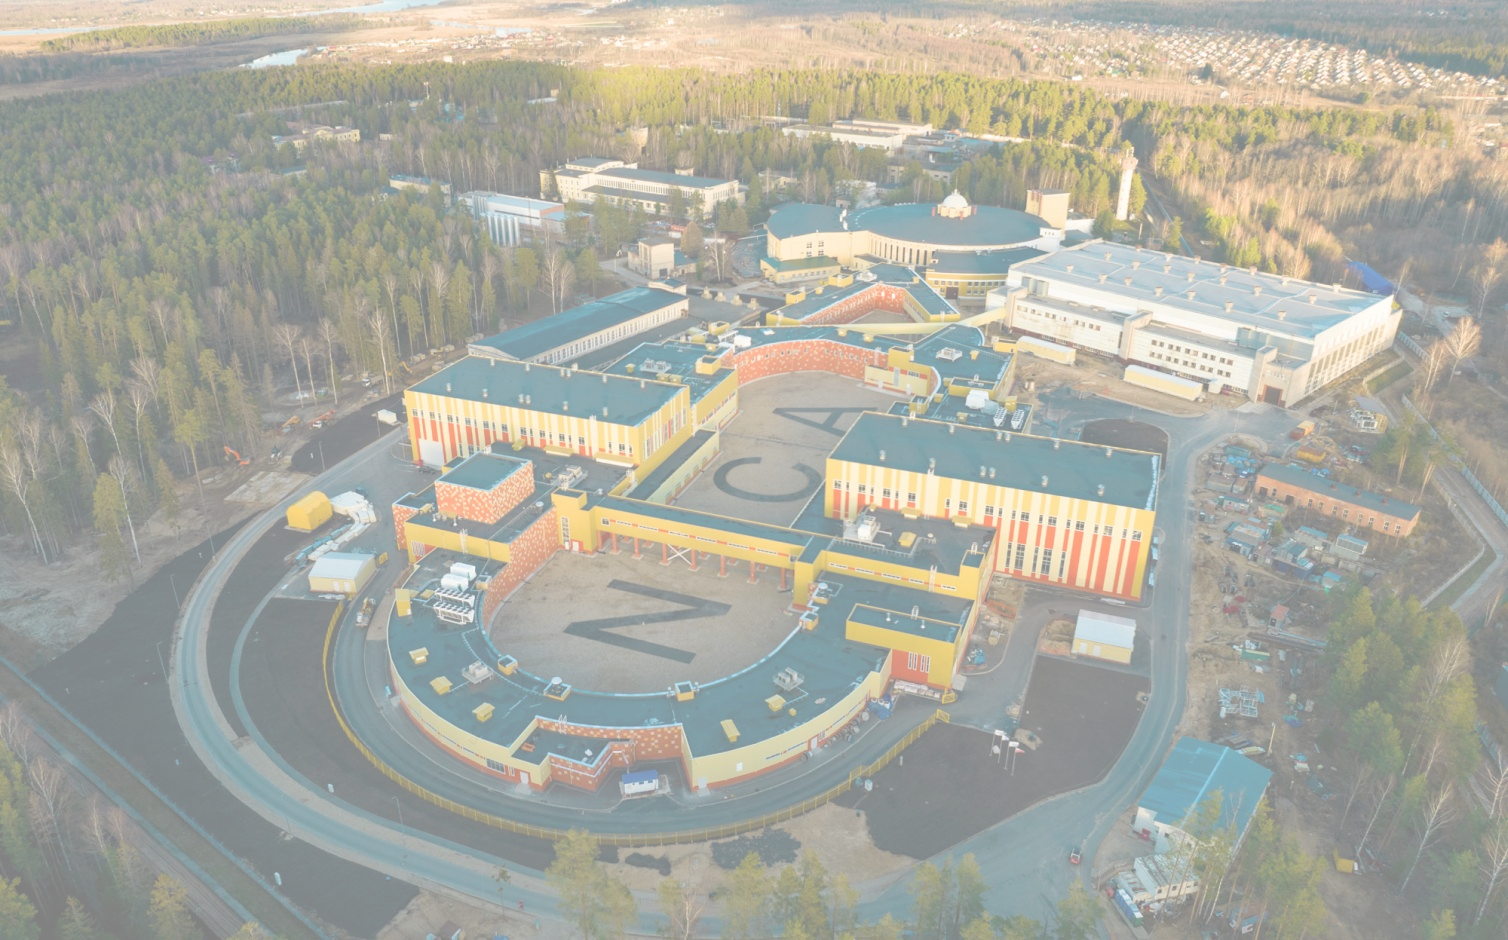
\includegraphics[width=\paperwidth]{nica2023_trans.png}}
% Disable logo
\logo{}

\begin{frame}
	\titlepage % Output the title slide, automatically created using the text entered in the PRESENTATION INFORMATION block above
\end{frame}

% Clear background
\usebackgroundtemplate{}
% Enable logo
\logo{
\includegraphics[width=1cm]{logo.eps}}

% Switch to Theme III
%\setbeamercolor{section in head/foot}{fg=scisGold, bg=white}
%\setbeamercolor{title in head/foot}{fg=white, bg=scisGold}
%\setbeamercolor{headline}{fg=scisGold, bg=white} 

%---------------------------------------------------------
%	TABLE OF CONTENTS SLIDE
%---------------------------------------------------------
% References sections and subsections, specified with the standard \section and \subsection commands. If you want to display all sections and subsections on one slide, just use \tableofcontents. If you want to just display each section one at a time (in subsequent slides) use \tableofcontents[pausesections].

\begin{frame}
	\frametitle{Оглавление} % Slide title, remove this command for no title
	\tableofcontents % Output the table of contents (all sections on one slide)
	%\tableofcontents[pausesections] % Output the table of contents (break sections up across separate slides)
\end{frame}
%---------------------------------------------------------
%	PRESENTATION BODY SLIDES
%---------------------------------------------------------
\section{Дуальная структура} % Note all sections and subsections are automatically placed in your table of contents

%------------------------------------------------
\begin{frame}
    \frametitle{Дуальная структура}
\par Двухцелевая (Дуальная) магнитооптическая структура, предназначенная для ускорения как тяжёлых ионов (например, золота), так и лёгких поляризованных протонов и дейтронов.
 \newline
 \par Гибкость настройки параметров структуры позволяет адаптировать её для работы с частицами, имеющими различные соотношения заряда к массе.
 \newline
 \par В комплексе NICA двойная магнитооптическая структура открывает перспективу ускорения как тяжелых ионов, таких как золото, так и легких частиц, таких как протоны и дейтроны.
\end{frame}
%------------------------------------------------
\section{Легкие частицы}

\begin{frame}
	\frametitle{Особенности ускорения легких частиц}
\par В классической регулярной структуре критическая энергия приблизительно равна бетатронной частице $\gamma_{\text{tr}}\simeq\nu_{\text{s}}$ и не зависит от типа частиц.
\newline
\par При одинаковой магнитной жесткости максимальная энергия для легких частиц больше, чем для тяжелых ионов, из-за их отношения заряда к массе. Это означает, что тяжелоионная структура, оптимизированная для работы с определенной критической энергией, потребует преодоления при работе с легкими частицами.
\end{frame}

%------------------------------------------------
\begin{frame}
	\frametitle{Критическая энергия}
     	Коэффициент уплотнения орбиты (momentum compaction factor)
     \small \begin{equation}
     	\alpha=\frac{1}{{\gamma_{\textrm{tr}}}^2}=\frac{1}{C}\int_{0}^{C}{\frac{D\left(s\right)}{\rho\left(s\right)}ds}
     \end{equation} \normalsize 	
     	Частота продольных колебаний пропорциональна коэффиценту проскальзывания (slip-factor)
	\begin{equation}
		 \omega_s\ \sim \eta, \quad \eta=\eta_0=1/\gamma_{tr}^2-1/\gamma^2
	 \end{equation} \normalsize 	
	При приближении энергии критической нарушается адиабатичность продольного фазового движения, а также значительное воздействие нелинейного эффекта более высоких порядков разброса импульса
	 
\end{frame}

%------------------------------------------------
\begin{frame}
	\frametitle{Суперпериодическая модуляция}
     Уравнение дисперсионной функции с бипериодической фокусировкой
         \small \begin{equation}
	   \frac{d^2D}{ds^2}+\left[K(s)+\varepsilon k(s)\right]D=\frac{1}{\rho(s)}
	 \end{equation} \normalsize 	
\small \begin{equation}
\alpha_{\text{s}}=\frac{1}{\nu^2_{x, \text {arc}}}\left\{1+\frac{1}{4}\left(\frac{\bar{R}_{\text {arc}}}{\nu_{x, \text {arc}}}\right)^4 \sum_{k=-\infty}^{\infty} \frac{g^2_k}{\left(1-k S / \nu_{x, \text {arc}}\right)\left[1-\left(1-k S / \nu_{x, \text {arc}}\right)^2\right]^2} \cdots\right\}
\end{equation} \normalsize 	
	\begin{figure}[h!]
		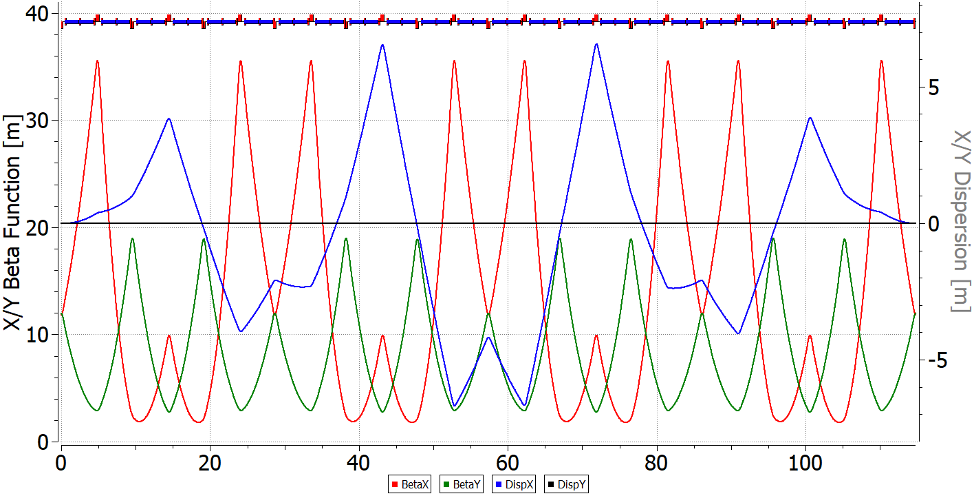
\includegraphics[width=6.5cm]{images/resonant_arc}
		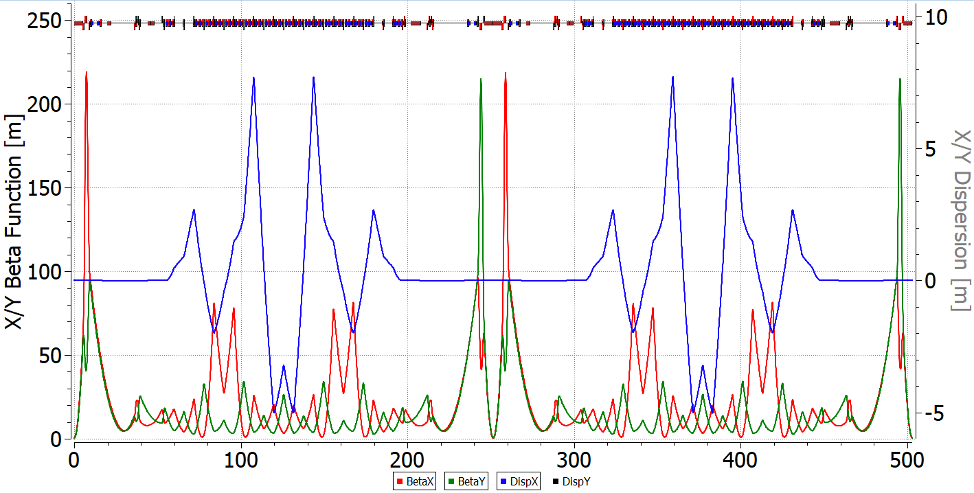
\includegraphics[angle=0, width=6.5cm]{resonant}
                \label{Figure 1}
	\end{figure}
	
	                
	

	 
\end{frame}
%------------------------------------------------
\section{Тяжелоионная мода}
%------------------------------------------------

\begin{frame}
	\frametitle{Время жизни пучка}
	
\begin{columns}[t]
	\begin{column}{0.5\textwidth}
\par Временная эволюция эмиттанса и разброса импульса при наличии процессов охлаждения

\small \begin{equation}
\begin{aligned}
& \dv{\varepsilon}{t}=\underbrace{-\frac{1}{\tau_{\text{tr}}} \cdot \varepsilon}_{\text {cooling}}+\underbrace{\left(\dv{\varepsilon}{t}\right)_{\text{IBS}}}_{\text{heating}} \\
& \dv{\delta^2}{t}=\underbrace{-\frac{1}{\tau_{\text{long}}} \cdot \delta^2}_{\text {cooling}}+\underbrace{\left(\dv{\delta^2}{t}\right)_{\text {IBS}}}_{\text {heating}} \\
&
\end{aligned}
\end{equation} \normalsize 	
	 \end{column}
	 \begin{column}{0.5\textwidth}
	 \par Темп охлаждения в отсутствии шума
	  	\small \begin{equation}
	 	\frac{1}{\tau_{\text{tr}}}=\frac{W}{N}\frac{\left(1-1/{M_{\text{pk}}}^2\right)^2}{M_{\text{kp}}}
	 	\end{equation} \normalsize 
	\par Коэффициент перемешивания (mixing factors)
	\par Пикап-киккер, киккер-пикап
	  	\small \begin{equation}
		\begin{aligned}
		M_{\text{pk}}&=\frac{1}{2\left(f_{\text{max}}+f_{\text{min}}\right)\eta_{\text{pk}}T_{\text{pk}}\delta} \\
		M_{\text{kp}}&=\frac{1}{2\left(f_{\text{max}}-f_{\text{min}}\right)\eta_{\text{kp}}T_{\text{kp}}\delta}
		\end{aligned}
	 	\end{equation} \normalsize 
          \end{column}
\end{columns}

\end{frame}

%------------------------------------------------
\begin{frame}
	\frametitle{Комбинированная структура}
\begin{columns}[t]
        \begin{column}{0.5\textwidth}
\par В случае “комбинированной” структуры одна арка регулярная, в то время как другая использует резонансную модуляцию.

\small \begin{equation}        
\eta_{\text{pk}}=1/\gamma_{\text{tr}}^2-1/\gamma^2
\end{equation} \normalsize 
\small \begin{equation}        
\eta_{\text{kp}}=-1/\gamma_{\text{tr}}^2-1/\gamma^2
\end{equation} \normalsize 

\par Резонансную арку можно получить из регулярной, введя дополнительное семейство фокусирующих квадруполей.

        \end{column}
        \begin{column}{0.5\textwidth}
            \begin{figure}[t]
                \centering
                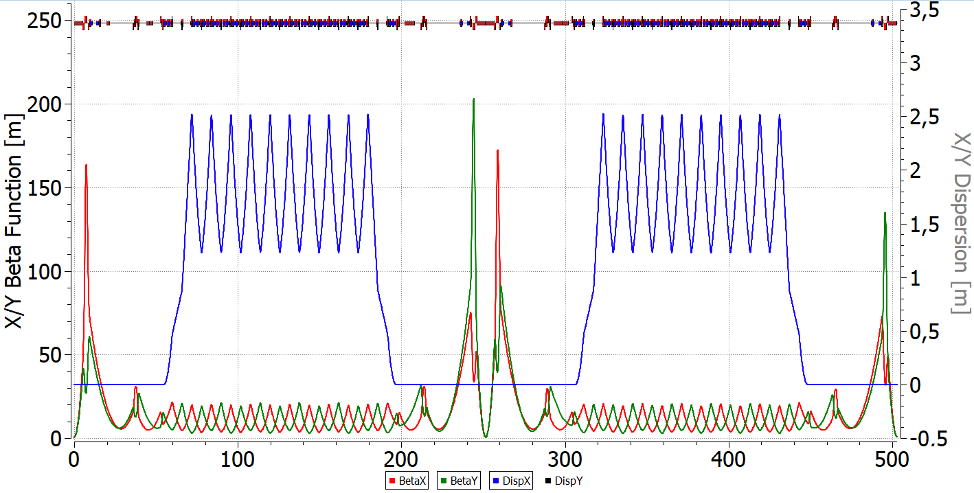
\includegraphics[width=6cm]{regular}
                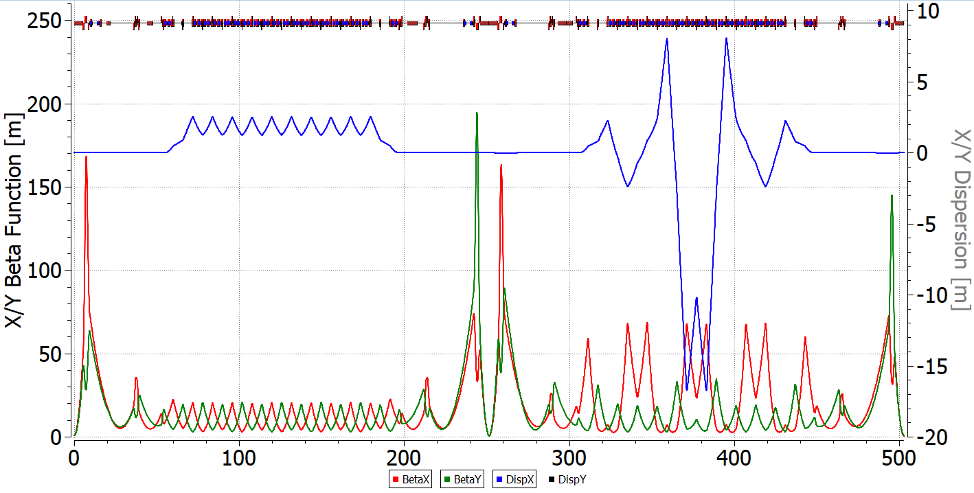
\includegraphics[width=6cm]{combined}
                \label{fig:structures}
            \end{figure}
        \end{column}
    \end{columns}
\end{frame}

%------------------------------------------------
\begin{frame}
	\frametitle{Стохастическое охлаждение}
	\begin{figure}[h!]
		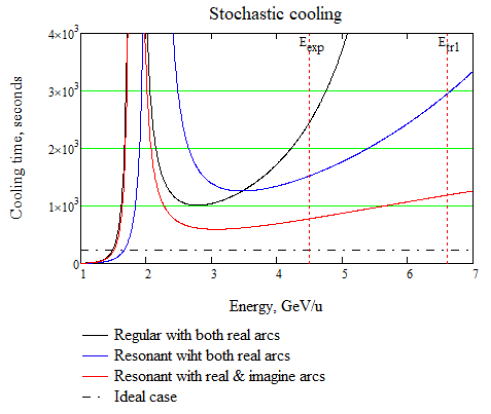
\includegraphics[width=6cm]{images/SC}
		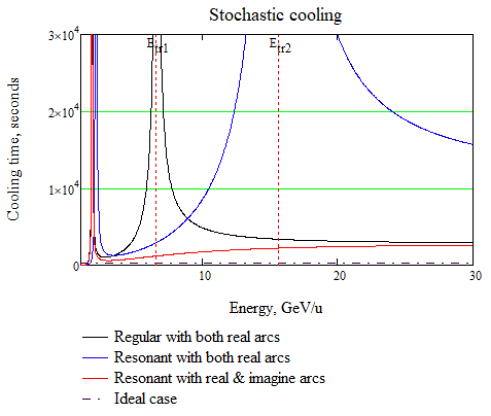
\includegraphics[width=6cm]{images/SC_wide}
                \label{Figure 1}
	\end{figure}
\end{frame}


%------------------------------------------------
\begin{frame}
	\frametitle{Внутрипучковое рассеяние}
\begin{center}
Темп внутрипучкового рассеяния	
\end{center}

\small \begin{equation}
\frac{1}{\tau_{\text{IBS}}}=\frac{\sqrt{\pi}}{4} \frac{c Z^2 r_p^2 L_{\text{C}}}{A} \cdot \frac{N}{C_{\text{orb}}} \cdot \frac{\left\langle\beta_x\right\rangle}{\beta^3 \gamma^3 \varepsilon_x^{5 / 2}\left\langle\sqrt{\beta_x}\right\rangle}\left(\left\langle\frac{D_x^2+\dot{D}_x^2}{\beta_x^2}\right\rangle-\frac{1}{\gamma^2}\right)
\end{equation} \normalsize

            \begin{figure}[h!]
                \centering
                % \caption{Hawkins et al, 2015}
                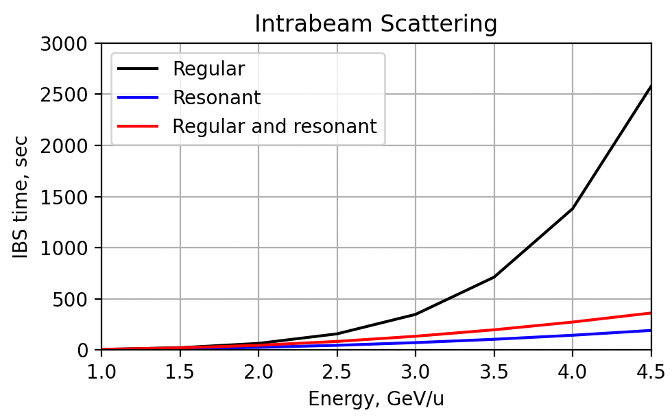
\includegraphics[width=6cm]{images/IBS}
                \label{fig:ibs}
            \end{figure}
	
\end{frame}
%------------------------------------------------
\section{Заключение}

%------------------------------------------------
\begin{frame}
	\frametitle{Основные параметры структур}

\begin{table}
\begin{center}
\begin{tabular}{|l|c|c|c|} 
\hline
Структура & Регулярная & Резонансная & Комбинир. \\
\hline Частицы & ${ }_{79}^{97} \mathrm{Au}$ & $\mathrm{p}$, $\mathrm{~d}$ & $\mathrm{p}$, $\mathrm{~d}$ \\
\hline Энергия эксперимента, ГэВ/нуклон & 4.5 & 12.6 & 12.6 \\
\hline Критическая энергия $\gamma_{\mathrm{tr}}$  & 7 & 15 & $i$50 \\
\hline Глубина модуляции & - & 25 \% & 45 \% \\
\hline Время охлаждения при 4.5 ГэВ, c & 2500 & 1500 & 800 \\
\hline Время ВПР при 4.5 ГэВ, c & 2500 & 400 & 250 \\
\hline
\end{tabular}
\end{center}
\label{tab:dual}
\end{table}

\end{frame}

\begin{frame}
	\frametitle{Заключение}
	
\par Гибкость дуальной структуры заключается в сочетании подходов, позволяющих обеспечивать контроль над ВПР для тяжёлых частиц и стабилизировать пучок при переходе через критическую энергию для лёгких частиц. 
\newline
\par Такой подход делает структуру универсальной для проведения коллайдерных экспериментов.
	
\end{frame}

\begin{frame}
	\frametitle{Благодарность}
	\begin{center}
		Спасибо за внимание!
	\end{center}
	
\end{frame}


\end{document}
